\documentclass{exam}

\usepackage{units} 
\usepackage{graphicx}
\usepackage[fleqn]{amsmath}
\usepackage{cancel}
\usepackage{float}
\usepackage{mdwlist}
\usepackage{booktabs}
\usepackage{cancel}
\usepackage{polynom}
\usepackage{caption}
\usepackage{fullpage}
\usepackage{xfrac}
\usepackage{enumerate}

\newcommand{\degree}{\ensuremath{^\circ}} 
\everymath{\displaystyle}

\printanswers

% \begin{figure}[H]
%   \centering
%   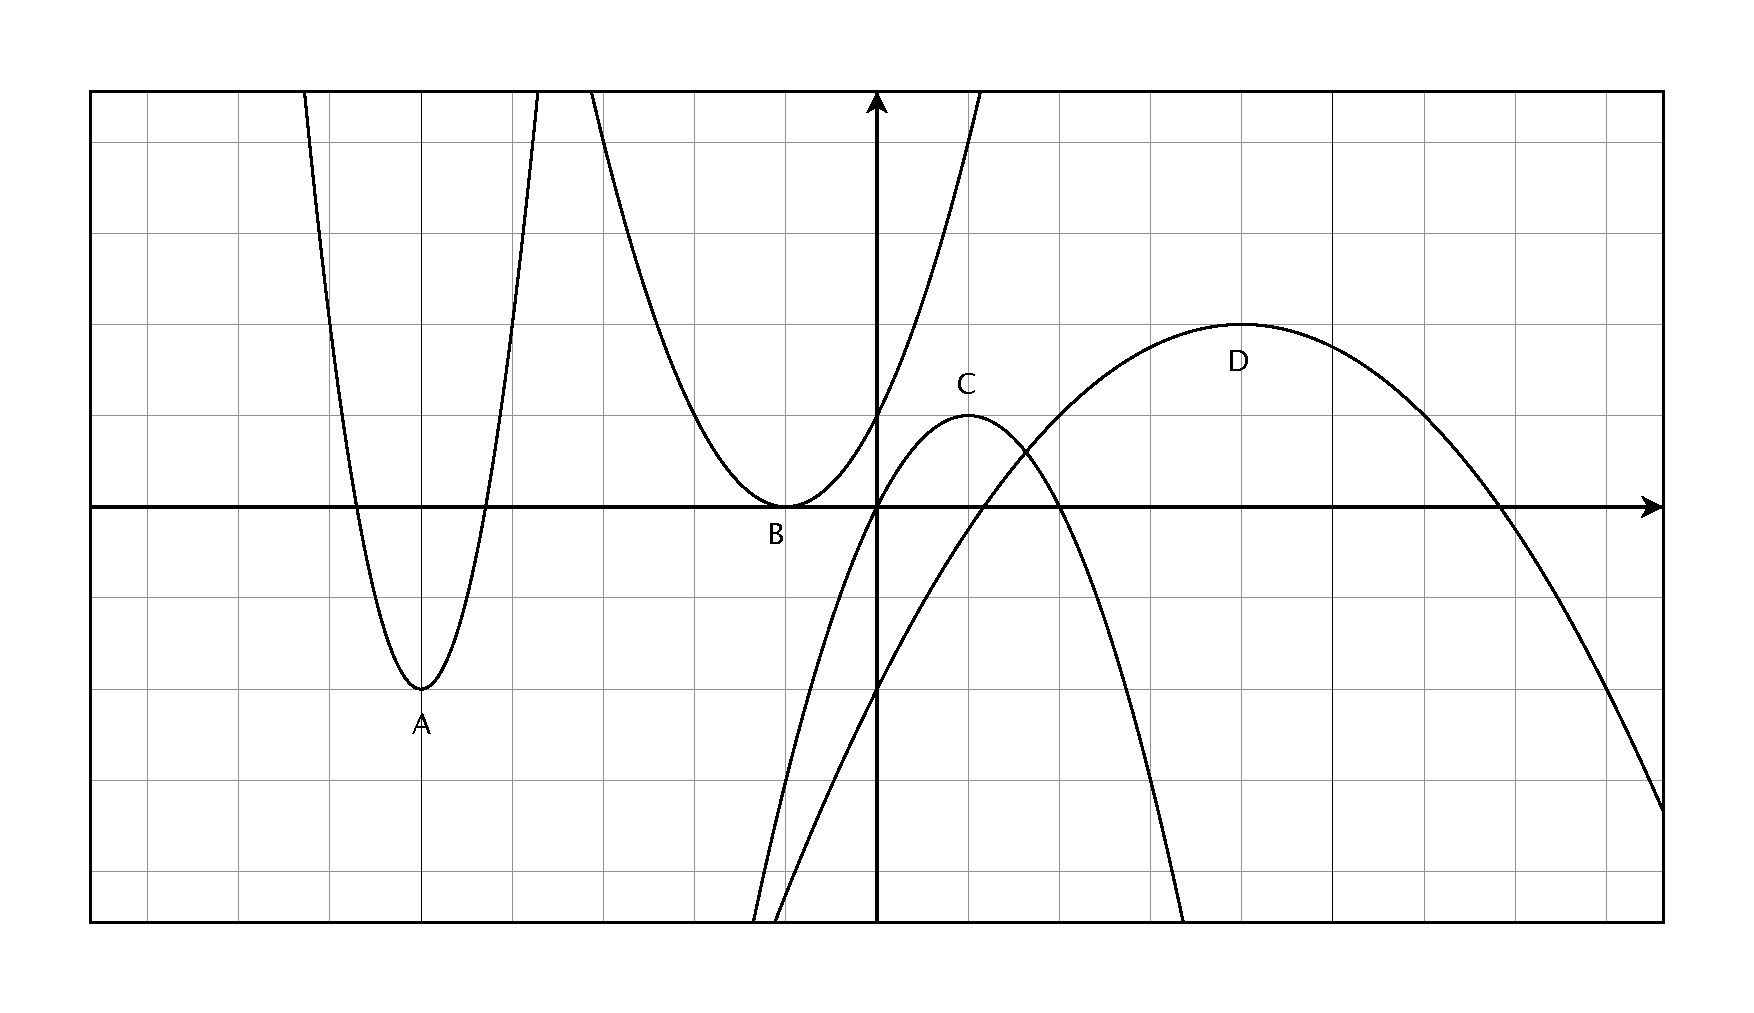
\includegraphics[scale=.3]{problem_7.eps}
%   \caption*{Problem 7}
% \end{figure}

% \begin{tabular}{cc}
% \toprule
% period & amplitude \\
% \midrule
%   $\pi$ & $2$ \\
% \bottomrule
% \end{tabular}

\title{Math 141 Notes \\ Section 2.6-2.7}
\date{February 13, 2013}

\begin{document}

\maketitle
\tableofcontents

\section{Proof of the Day}
Do even/odd function proofs from HW 3.  Showing an example ($x^2 + x^4$ is even, for example) is not a proof.

  \begin{description}
    \item[75]
      If $f$ and $g$ are both even, $f(-x) = f(x)$ and $g(-x) = g(x)$.  
      \begin{align*}
        (f + g)(-x) &= f(-x) + g(-x) \\
          &= f(x) + g(x) \\
          &= (f + g)(x) \\
      \end{align*}
      So in this case, $(f + g)(x)$ is even.

      If $f$ and $g$ are both odd, $f(-x) = -f(x)$ and $g(-x) = -g(x)$.  
      \begin{align*}
        (f + g)(-x) &= -f(x) + (-g(x)) \\
          &= - (f(x) + g(x)) \\
          &= -(f + g)(x) \\
      \end{align*}
      So in this case, $(f + g)(x)$ is odd.

      If $f$ is even and $g$ is odd, $f(-x) = f(x)$ and $g(-x) = -g(x)$.  
      \begin{align*}
        (f + g)(-x) &= f(x) + (-g(x)) \\
          &= f(x) - g(x) \\
      \end{align*}
      So in this case, $(f + g)(x)$ is neither even nor odd.

    \item[76]
      If $f$ and $g$ are both even, $f(-x) = f(x)$ and $g(-x) = g(x)$.  
      \begin{align*}
        (f \cdot g)(-x) &= f(-x) \cdot g(-x) \\
          &= f(x) \cdot g(x) \\
          &= (f \cdot g)(x) \\
      \end{align*}
      So in this case, $(f \cdot g)(x)$ is even.

      If $f$ and $g$ are both odd, $f(-x) = -f(x)$ and $g(-x) = -g(x)$.  
      \begin{align*}
        (f \cdot g)(-x) &= -f(x) \cdot (-g(x)) \\
          &= f(x) \cdot g(x) \\
          &= (f \cdot g)(x) \\
      \end{align*}
      So in this case, $(f \cdot g)(x)$ is even.

      If $f$ is even and $g$ is odd, $f(-x) = f(x)$ and $g(-x) = -g(x)$.  
      \begin{align*}
        (f \cdot g)(-x) &= f(x) \cdot (-g(x)) \\
          &= - f(x) \cdot g(x) \\
      \end{align*}
      So in this case, $(f \cdot g)(x)$ is odd.
  \end{description}

\section{Min/Max Problems}

\begin{enumerate}
  \item Find the dimensions of a rectangle with perimeter $\unit[100]{m}$ whose area is as large as possible.

    \begin{solution}
      \begin{align*}
        2x + 2y &= 100 \\
        \\
        A(x) &= -x^2 + 50x \\
        x &= 25 \\
      \end{align*}
    \end{solution}

  \pagebreak

  \item Show that of all the rectangles with a given perimeter, the one with the largest area is a square.

    \begin{solution}
      \begin{align*}
        2x + 2y &= P \\
        \\
        A(x) &= -x^2 + \frac{Px}{2} \\
        x &= \frac{P}{4} \\
      \end{align*}
    \end{solution}

  \item A farmer with 750 feet of fence wants to enclose a rectangular area divided into four pens.  What is the largest
    possible total area?

    \begin{solution}
      \begin{align*}
        2x + 5y &= 750 \\
        A       &= \frac{-2x^2}{5} + 150x \\
        \\
        x       &= \unit[187.5]{ft} \\
        y       &= \unit[75]{ft} \\
      \end{align*}
    \end{solution}

  \item Find the point on the line $y = 2x + 1$ that is closest to the origin.

    \begin{solution}
      Optimize distance squared:
      \begin{align*}
        d(x) &= x^2 + (2x + 1)^2 \\
        &= 5x^2 + 4x + 1 \\
        \\
        x &= - \frac{2}{5} \\
        y &= \frac{1}{5} \\
      \end{align*}
    \end{solution}

  % \item Find the point on the line $6x + y = 9$ that is closest to the point $(-3, 1)$.

  \pagebreak

  \item 
    Find the number of units that produces the maximum revenue:
    \[
      R = 900x - 0.1x^2
    \]
    where R is the total revenue and $x$ is the number of units sold.

  \item
    A manufacturer has daily production costs of:
    \[
      C =  0.25x^2 - 10x + 800 
    \]
    where C is the total cost and $x$ is the number of units produced.  How many units should be produced each day to
    yield a minimum cost.

  \item Find the dimensions of the rectangle of largest area that can be inscribed in an equilateral triangle of side
    $L$ if one side of the rectangle lies on the base of the triangle.

    \begin{solution}
      First find the equation of the line that makes up one side of the triangle:
      \begin{itemize*}
        \item y-intercept = height = $\frac{L \sqrt{3}}{2}$
        \item slope = $- \sqrt{3}$
        \item equation: $y = - \sqrt{3} x + \frac{L \sqrt{3}}{2}$
      \end{itemize*}

      The equation to optimize is: $A(x) = -2 \sqrt{3} x^2 + L\sqrt{3}x$.

      The solution is: $x = \frac{L}{4}$ and $y = \frac{\sqrt{3} L}{4}$.
    \end{solution}

  \pagebreak

  \item 
    A track contains a rectangular region with a semicircle on each end.  The perimeter is to be a 200 meter running
    track.

    \begin{enumerate}[a]
      \item Find the radius of the semicircular parts.  Determine the distance, in terms of $y$ around the two
        semi-circular parts of the track.

        \begin{solution}
          $\pi y$
        \end{solution}

      \item Use the result of part (a) to write an equation, in terms of $x$ and $y$ of the distance traveled in one lap
        around the track.  Solve for $y$.
        \begin{solution}
          \begin{align*}
            200 &= 2x + \pi y \\
            y &= \frac{200 - 2x}{\pi} \\
          \end{align*}
        \end{solution}

      \item Use the result of part (b) to write the area, $A$ of the rectangular region as a function of $x$.  What
        dimensions will produce the maximum area of the rectangle?
        \begin{solution}
          \begin{align*}
            A &= \frac{1}{\pi} (-2x^2 + 200x ) \\
            x &= 50 \\
            y &= \frac{100}{\pi} \\
          \end{align*}
        \end{solution}
    \end{enumerate}
\end{enumerate}

\pagebreak

\section{Combining Functions}

\subsection{Algebra of Functions}
\subsubsection{Notes}

\begin{align*}
  (f + g)(x)                    &= f(x) + g(x) \\
  (f - g)(x)                    &= f(x) - g(x) \\
  (f \cdot g)(x)                &= f(x) \cdot g(x) \\
  \left( \frac{f}{g} \right)(x) &= \frac{f(x)}{g(x)} \\
\end{align*}

\begin{itemize}
  \item Domain is the intersection of the original domains, excluding values where $g(x) = 0$ in the division case.
  \item Draw machine picture.
\end{itemize}

\subsubsection{Examples}

Find $(f + g)(x)$, $(f - g)(x)$, $(f \cdot g)(x)$, and $\left( \frac{f}{g} \right)(x)$ and their domains.

\begin{enumerate}
  \item $f(x) = x^2$; $g(x) = x + 1$

  \item $f(x) = \sqrt{x^2 - 9}$; $g(x) = \sqrt{x + 2}$

  \item $f(x) = \frac{1}{x}$; $g(x) = \frac{x}{x + 1}$

\end{enumerate}

\subsection{Composition of Functions}
\subsubsection{Notes}

\[
  (f \circ g)(x) = f(g(x))
\]

\begin{itemize}
  \item Domain is the values in the domain of $g$ such that $g(x)$ is in the domain of $f$.

  \item Draw machine picture and linked domain pictures.

\end{itemize}

\subsubsection{Examples}

\begin{enumerate}
  \item If $f(x) = 2x + 1$ and $g(x) = x^2 + 2$, evaluate:
    \begin{enumerate}[a]
      \item $f(g(0))$

      \item $g(f(0))$

      \item $f(f(0))$

      \item $g(g(0))$

    \end{enumerate}

  \item Find $(f \circ g)(x)$, $(g \circ f)(x)$, $(f \circ f)(x)$, $(g \circ g)(x)$, and their domains.
    \begin{enumerate}[a]
      \item $f(x) = 2x + 1$; $g(x) = 3x - 1$

      \item $f(x) = x^2 + 1$; $g(x) = \sqrt{x}$

      \item $f(x) = \sqrt{x - 1}$; $g(x) = x^2 - 3$
    \end{enumerate}

  \item If $f(x) = ax + b$ and $g(x) = cx + d$, When does;
    \begin{itemize*}
      \item $(f \circ g)(x) = (g \circ f)(x)$?
      \item $(f \circ g)(x) = f(x)$?
      \item $(f \circ g)(x) = g(x)$?
    \end{itemize*}

  \item Express $h(x) = \frac{1}{(x - 2)^2}$ as a composition of two functions.
    \begin{solution}
      \begin{align*}
        f(x) &= \frac{1}{x^2} \\
        g(x) &= x - 2 \\
      \end{align*}
    \end{solution}

  \item Express $h(x) = \sqrt[3]{x^2 - 1}$ as a composition of two functions.

  \item Sand is pored into a conical pile whose radius and height are always equal, although both increase with time.
    The height of the pile $\unit[t]{seconds}$ after pouring begins is given by $h(t) = \unit[10 + 0.25t]{ft}$.  Express the
    volume of the pile as a function of $t$.

    The volume of a cone is $v = \frac{1}{3} \pi r^2 h$.

    \begin{solution}
      \begin{align*}
         v &= \frac{1}{3} \pi h^3 \\
       &= \frac{1}{3} (10 + 0.25t)^3 \\
      \end{align*}
    \end{solution}

  \item Tax Rates
    Alice has a mortgage and 401(k) plan.  She is in the 30\% tax bracket and pays 6\% Social Security tax on the first
    \$100,000 of her income, which is more than \$100,000.  She also spends 20\% of her income on taxable items which
    are taxed by the WA state sales tax of 10\%.

    Bob rents, is in the 25\% tax bracket and doesn't have a 401(k) plan.  He makes less than \$100,000 and spends 50\%
    of his income on taxable items.

    Find functions for each person's tax rate.  If Alice makes \$150,000 and Bob makes \$50,000, find their tax rates.

    \begin{solution}
      \begin{itemize}
        \item Alice's taxable income is: $A(x) = x - 15000 - 15000$
        \item Alice's tax, as a function of income is: $T(i) = 0.3i + 0.02i + 6000 = 0.32i + 6000$
        \item Alice's tax rate is $R \circ T \circ A$.
        \item Bob's taxable income is: $B(x) = x$
        \item Bob's tax rate is: $T(i) = 0.25i + 0.05i + 0.06i = 0.36i$
      \end{itemize}

      \begin{itemize*}
        \item Alice's effective tax rate is 30\%.
        \item Bob's effective tax rate is 36\%.
      \end{itemize*}
    \end{solution}
    
  \item A spherical balloon is inflated so that its radius at the end of $\unit[t]{seconds}$ is 
    \[
      r(t) = \unit[3 \sqrt{t} + 5]{cm}
    \]

    Express the volume and the surface area as functions of time.

    \begin{solution}
      \begin{align*}
        V(t) &= \frac{4}{3} \pi r^3 \\
        A(t) &= 4 \pi r^2 \\
      \end{align*}
    \end{solution}

\end{enumerate}

\section{Miscellaneous}

Talk to Jeff Grote about 
\begin{itemize*}
  \item piecewise defined functions
  \item sign charts
  \item use \verb+[] or ()+ instead of \verb+{}+ for ranges
\end{itemize*}

\end{document}

